\chapter{Multiphase Formulation and Pressure Drop}

The focus of this section is to introduce the reader to the modelling of multiphase flow in general, liquid-gas flows in particular and the prediction of pressure drop and void specifically.
The main objective is to provide the reader with the basic fundamentals that are needed to formulate the balance equations for multiphase flow as well as the associated constitutive relations and then employ them in the practical prediction of pressure drop in a closed conduit as the first example of their usefulness.
As in other sections this is a diverse subject and more detailed discussions of these topics are provided by a number of individuals; e.g., Collier, 1981; Wallis, 1979; Bergles et al., 1981; Hsu and Graham, 1977; and Ishii, 1974.

\begin{figure}[h]
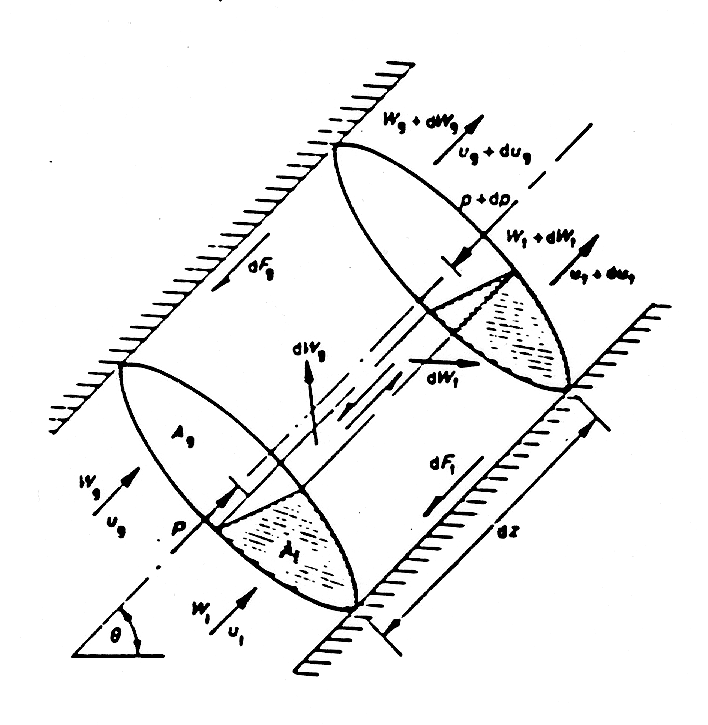
\includegraphics[width=0.5\textwidth]{images/vertical_tube_heat_addition.png}
\caption{Conceptual Picture of 1-D Two-Phase Flow in a Tube}
\label{fig:vertical_tube_heat_addition}
\end{figure}

Once the concept of flow patterns for multiphase flow has been introduced, one must develop the governing equations which account for the conservation of mass and energy and the transfer of momentum.
Consider the case of steam-water flow in a vertical tube with heat addition at the wall boundary (Figure \ref{fig:vertical_tube_heat_addition}).
In reality the phases are not exactly in thermodynamic and mechanical equilibrium; i.e., if the channel geometry is variable and the flow rate or heat addition rate is changing rapidly with time or space, then the velocity, temperature and pressure of the two-phases are not necessarily the same at a given spatial position in the channel.
For certain conditions one may be able to model the multiphase flow and assume that some or all of these potential variables may be equal between the phases.
To cover a broad range of applications a number of models have been developed.
We consider three general types of multiphase flow models, the homogeneous flow model, separated flow model and two fluid model.
Table \ref{table:two_phase_summary} gives a brief summary of important dimensionless groups that can be used to determine model applicability.
\renewcommand*\arraystretch{1.5}
\ctable[
	caption = Important Dimensionless Variables in Multiphase Flow\tmark,
	mincapwidth = \textwidth,
	label = table:two_phase_summary
	]{l c c}{
	\tnote{In this list the characteristic length, $L$, could be the diameter of the channel, or the length scale of the dispersed phase (bubble diameter) depending on the specific application.}
	\tnote[b]{This dimensionless constant is a useful property length scale for multiphase flow calculations compared to bubble diameter when the channel or chamber size is large.}
	}{											\FL	
Atwood Ratio & At & $\frac{p_2-p_1}{p_2+p_1}$ 	\NN
Fourier Number & Fo & $\frac{a^2}{L^2}$ 		\NN
Froude Number & Fr & $\frac{V^2}{g L}$ or $Fr^* = \frac{Fr}{At} = \left(\frac{p_2+p_1}{p_2-p_1}\right)\frac{V^2}{gL}$ \NN
Laplace Constant\tmark[b] & A & $\sqrt{\frac{\sigma}{\Delta \rho g}}$ \NN
Hem Mach Number & M & $M^2 = G^2\left[\frac{x_1}{\rho_1^2 C_1^2}+\frac{x_2}{\rho_2^2 C_2^2}\right]$ \NN
Martinelli Number & X & $X^2 = (\frac{x_1}{x_2})^{1.8}(\frac{\rho_2}{\rho_1})(\frac{\mu_1}{\mu_2})^{0.2}$ \NN
Prandtl Number & Pr & $\frac{C_p \mu}{k}$\NN
Reynolds Number & Re & $\frac{\rho V L}{\mu}$\NN
Weber Number & We & $ \frac{\rho V^2 L}{\sigma}$ \LL
}

\section{Homogeneous Equilibrium Model}

In the homogeneous equilibrium model (HEM) one assumes that the velocity, temperature, and pressure between the phases or components are equal.
This assumption is based on the belief that differences in these three potential variables (and chemical potential if chemical reactions are considered) will promote momentum, energy, and mass transfer between the phases rapidly enough so that equilibrium is reached.
For example, when one phase is finely dispersed in another phase generating large interfacial area, under certain circumstances this assumption can be made; e.g., bubbly flow of air in water or steam in water at high pressures.
The resulting equations resemble those for a pseudo-fluid with mixutre properties and an equation of state which links the phases to obtain these mixture thermodynamic properties.
Whenever the HEM model is used it is advisable to check the validity of the equilibrium assumptions by using more accurate theoretical models for comparison.
For example, rapid acceleration or pressure changes cannot be always accurately modelled with the HEM model; i.e., discharge of flashing vapor-liquid mixtures, or shock wave propagation through a multiphase medium.
This is especially true when the pressure change is large when compared to the ambient pressure, or any of the driving potentials are large relative to their reference values.
Such a 'rule-of-thumb' is very crude and one must carefully consider the timescales for equilibration of these driving potentials with allowable characteristic times for the problem of interest.

\ctable[
	caption = Homogeneous Equilibrium Model Governing Equations\tmark,
	mincapwidth = \textwidth,
	label = {table:hem_governing_equations}
	]{l l r}{
	\tnote{In the table it is assumed that only two phases are present, but this can be easily be extended for more phases or components.}
	}{																\FL	
Mass 					& $\frac{\partial}{\partial t}\left(\rho A\right) = -\frac{\partial}{\partial z}\left(\rho A v\right)$  								& (1) 		\NN
Energy 					& $\frac{\partial(\rho A e)}{\partial t} = -\frac{\partial}{\partial z}(\rho A v(e + Pv)) + q^{''}_{w} P_{w} + v \tau_w P_{w} + \frac{\partial}{\partial z}(k A \frac{\partial T}{\partial z}) $ 		& (2)		\NN
Momentum 				& $\frac{\partial(A v)}{\partial t} = - \frac{\partial(\rho A v^2)}{\partial z} - \rho g A sin(\theta) - \tau_w P_w - \frac{\partial(P A ) }{\partial z}$ 			& (3) 		\NN
Equation of State 		& Properties $ = f(\rho, u)$	& (4)		\NN
\underline{Constituitive Relations} &  								& 			\NN
						& $\tau_w = f(\rho, v, D_H, \mu)$	& (5)		\NN
						& $q^{''}_w = h(T_w - T)$		& (6)		\NN
						& $A = f(z, t)$					& (7)		\NN
\underline{Definitions} 			& 	 							& 			\NN
Total Energy 			& $e \cong	 u + \frac{v^2}{2} + g z sin(\theta)$ 	& (8)		\NN
Mixture Density 		& $\rho \cong \alpha_1 \rho_1 + \alpha_2 \rho_2 $	& (9)		\NN
Internal Energy 		& $u \cong x_1 u_1 + x_2 u_2 $	& (10)		\NN
Specific Volume 		& $\nu \cong x_1 \nu_1 + x_2 \nu_1 = \frac{1}{\rho}$		& (11)		\NN
Thermal Conductivity 	& $k \cong f(k_1, k_2, \alpha_1, \alpha_2) $ & (12)		\NN
Viscosity 				& $\mu \cong f(\mu_1, \mu_2, \alpha_1, \alpha_2)$	& (13)\LL
}

The governing equations for the HEM model are presented in Table \ref{table:hem_governing_equations} where the geometry has been chosen to be a one-dimensional channel inclined from the horizontal by a known angle, $\theta$, (Figure \ref{fig:vertical_tube_heat_addition}).
The microscopic equations have been averaged over the channel cross-sectional area using the techniques first proposed by Ishii (1974), leaving a partial differential equation in time, $t$, and the axial space dimension, $z$.
The definitions of the mixture thermodynamic properties (e.g., $\rho$, $u$, $v$) consider only two-phases but can be simply extended to more phases or components.
The extension to more than one-dimension is not as straight forward and one is referred to the general formulation of Bird, et al. (1960).
Note that the inclusion of the mixture thermodynamic properties can be followed from Table \ref{table:hem_governing_equations}.

The multiphase transport properties of viscosity and thermal conductivity ( $\mu$ , $k$) are another matter, because it is not clear how one should average their effect in an area-average, mass average or volume-average sense.
In many situations such as for pressure drop calculations the mixture transport properties have been arbitrarily averaged on a volume average or mass average basis, e.g.,

\begin{equation}
\mu = x_1 \mu_1 + x_2 \mu_2\quad \mathsf{or}\quad \mu = \alpha_1 \mu_1 + \alpha_2 \mu_2
\end{equation}

However, these averaging schemes are not exact and are usually empirically corrected by fitting coefficients to a set of experimental data.
In other situations the effect of multiphases are neglected and the liquid or gas property values for viscosity on the thermal conductivity are used, e.g., when the amount of liquid in the channel is large (low quality or void fraction), the viscosity can be taken to be that of the liquid.

\section{Seperated Flow Model}

In the separated flow model the restriction on equal phase velocities is relaxed and one now models the momentum exchange between the phases and the channel separately with different velocities, e.g., vapor and liquid velocities.
The relaxation of equal velocities is most important when the densities between the phases are quite different in the presence of a gravitational potential field or large pressure gradients.
Given a density difference, buoyancy effects tend to induce a drift velocity of the lighter phase in the heavier phase.
One measure of this density ratio is the Atwood ratio and is defined in Table \ref{table:two_phase_summary}.
One notices that as this density ratio approaches zero the HEM model would become more valid because the drift velocity would be reduced as the buoyancy of the lighter phase diminishes.
The remaining assumptions of equal temperatures and pressures between the phases are usually retained in most applications.
This is because it is usually felt the rates of mass and energy exchange are large enough to promote equilibrium.
Once again a check with a more detailed model is recommended as the analysis proceeds to verify this assumption.

The governing equations for the separated flow model are given in Table \ref{table:seperated_flow_model}.
Similar to Table \ref{table:hem_governing_equations} we use the 1-D area averaged formulation for two phases.
There are two important differences in the equations that one should notice.
First, there are now two momentum equations.
In each equation there appears a term which represents the friction force at the phase interface caused by the relative velocity between the phases.
If the equations are solved separately then one must develop a constitutive relation model for this momentum transfer term.
Second, the properties are not averaged exclusively using the void fraction and density of the phases, but require a separate constitutive relation (Eq. 10 in Table \ref{table:seperated_flow_model}) that relates the volume fraction to the flowing mass fraction.
Traditionally the separated flow model has been used primarily for calculating the pressure drop in a flow channel.
In this application the usual method of solution is to add the phase momentum equations and eliminate the need to model the interfacial shear stress, $\tau_i$.
Then one empirically correlates to obtain a model for the frictional pressure drop for the channel, $\tau_w$, and for the slip ratio, $\frac{v_2}{v_1}$, or velocity differences $(v_2-v_1)$ between the phases as a function of volume fraction and properties.
The model for $\tau_w$ is substituted back in the combined momentum equation and the algebraic correlation for $\frac{v_2}{v_1}$ or $(v_2-v_1)$ is used as a substitute for the second balance equation.
These types of models are described in more detail when one considers multiphase pressure drop.
The drift flux model is a special case of such models, because it is physically based as it predicts void fractions given velocity difference.

\ctable[
	caption = Separated Flow Model Governing Equations\tmark,
	mincapwidth = \textwidth,
	label = table:seperated_flow_model
	]{l l r}{
	\tnote{This table considers only two phases present. Also, the frictional (viscous and turbulent) dissipation term and the axial conduction term have been neglected similar to most applications.}
	}{																\FL	
Mass 					& $\frac{\partial}{\partial t}\left(\rho A\right) = -\frac{\partial}{\partial z}\left(\rho A v\right)$  								& (1) 		\NN
Energy 					& $\frac{\partial(\rho A e)}{\partial t} = -\frac{\partial}{\partial z}(\rho A v(e + Pv)) + q^{''}_{w} P_{w} + v \tau_w P_{w} + \frac{\partial}{\partial z}(k A \frac{\partial T}{\partial z}) $ 		& (2)		\NN
Momentum Phase 1		& $\frac{\partial(A v)}{\partial t} = - \frac{\partial(\rho A v^2)}{\partial z} - \rho g A sin(\theta) - \tau_w P_w - \frac{\partial(P A ) }{\partial z}$ 			& (3) 		\NN
Momentum Phase 2		& $\frac{\partial(A v)}{\partial t} = - \frac{\partial(\rho A v^2)}{\partial z} - \rho g A sin(\theta) - \tau_w P_w - \frac{\partial(P A ) }{\partial z}$ 			& (4) 		\NN
\underline{New Constituitive Relations} &  								& 			\NN
						& $\tau_w = f(\rho, v, D_H, \mu)$	& (5)		\NN
\underline{New Definitions} 			& 	 							& 			\NN
Total Energy 			& $e \cong	 u + \frac{v^2}{2} + g z sin(\theta)$ 	& (6)		\NN
Mixture Density 		& $\rho \cong \alpha_1 \rho_1 + \alpha_2 \rho_2 $	& (7)		\NN
Internal Energy 		& $u \cong x_1 u_1 + x_2 u_2 $	& (8)		\NN
Specific Volume 		& $\nu \cong x_1 \nu_1 + x_2 \nu_1 = \frac{1}{\rho}$		& (9)		\NN
Thermal Conductivity 	& $k \cong f(k_1, k_2, \alpha_1, \alpha_2) $ & (10)		\LL
}

\section{Two-Fluid Model}

The final type of multiphase model is the multiple fluid model (better known as the two fluid model designating two phases or components).
This model treats the general case of modelling each phase or component as a separate fluid with its own set of governing balance equations.
In general each phase has its own velocity, temperature and pressure.
The velocity difference as in the separated flow is induced by density differences.
The temperature differences between the phases is fundamentally induced by the time lag of energy transfer between the phases at the interface as thermal equilibrium is reached.
If the multiphase system involves rapidly changing flow conditions due to area changes in steady flow or transient conditions then the time lag for reaching thermal equilibrium between the phases may become significant in comparison to the characteristic time it takes for flow conditions to change.
One may estimate this condition by computing a characteristic Fourier number (Table \ref{table:two_phase_summary}) for the system under expected flow conditions.
Therefore, thermal nonequilibrium becomes important and one must include the possibility of a temperature difference by separate energy balances in a multiphase model for two or more separate fluids.

The modelling of pressure nonequilibrium is much more complex (Ishii, 1974).
The pressure difference between two phases is caused by three main effects: (1) pressure differences due to surface energy of a curved interface,(2) pressure differences due to mass transfer, and (3) pressure differences due to dynamic effects.
In the first case the simple existence of an interface (probably curved) requires from overall mechanical equilibrium that some pressure difference exist between the phases.
This pressure difference is proportional to the interfacial surface tension and inversely proportional to the radius of curvature ($\sim \frac{2\sigma}{r}$) and is usually quite small in most applications ( $ r > 100 \mu m$).
The second effect is noticeable when the mass flux due to phase change is large at the interface between the phases; e.g., large evaporation or condensation rates.
The final effect is caused by dynamics where one phase has a larger pressure relative to the other phase due to very rapid energy deposition or pressurization effects.
A common example of an induced dynamic pressure difference is the flow of a mixture of air bubbles and water through a converging-diverging nozzle.
If the rate of flow is high and the area change dramatic enough the liquid will depressurize quickly as it passes through the nozzle leaving the vapor bubbles at a higher pressure.
This dynamic pressure difference will cause the vapor bubbles to grow, overexpand and then oscillate around a new mean pressure.
This example takes on the second effect if the situation were steam bubbles in water since mass transfer would also be present.
The importance of pressure nonequilibrium between the phases is inversely proportional to the time scale of the rate of phase change or external pressure oscillations.
For most applications of two-fluid modelling this pressure nonequilibrium is usually neglected; i.e., only when the rate of phase change and pressure oscillation become of equal time scales does this nonequilibrium effect become important.
One way to estimate this is to compare the flow velocity to the speed of sound in the multiphase system (note that computing a mixture sound speed is not a straight forward task): i.e., only when the flow velocity approaches or exceeds the multiphase sound speed would the pressure nonequilibrium may be important.

The two-fluid model equations are given in Tables \ref{table:34}.
One should note that when a two-fluid model is used a number of interfacial transport coefficients ( $\gamma_i$, $\tau_i$, $q^{''}_i$, $P_i$) are defined and require constitutive relation models to complete the overall model.
This approach has an advantage in that the actual transport processes can be rigorously defined, however, the disadvantage is that one is required to model these kinetic processes in detail, which implies a much greater depth of experimental data and insight.

The usual method of modelling pressure differences between the fluids is to assume that the pressure is equal in both phases (Tables \ref{table:34}, Eq. 6).
If, as previously discussed, one finds that pressure nonequilibrium between the phases is important one must introduce a local constitutive relation which accounts for this pressure difference due to dynamic and interfacial effects.
For example, in research done with explosive boiling a local momentum equation (e.g., Rayleigh momentum equation) is used to model this difference in the pressure of the two fluids; this allows for dynamic pressure differences as well as the effect of surface tension and mass transfer.

The other required constitutive relations for interfacial transfer ( $\gamma_i$, $\tau_i$, $q^{''}_i$) are complicated functions of the fluid velocities and their local properties.
These kinetic models are also a strong function of the multiphase flow pattern.
The model one would develop for the interfacial shear stress or heat flux is significantly different for a dispersed flow pattern in contrast to a stratified flow pattern.
In fact, the interfacial models would be different if one had gas bubbles in a liquid versus liquid droplets in a gas.
For example in the former case one would find that the stable characteristic size of gas bubbles at low void fractions might be near the Taylor critical wavelength (dimensionless length $\frac{D}{A} \sim 2\pi$, Table \ref{table:two_phase_summary}) where as in the latter case the diameter would be determined from the critical Weber number ($We \sim 7-12$, Table \ref{table:two_phase_summary}) which is only partly related to Taylor instabilities.

The final point to make about all the multiphase models is how turbulence is included in the analysis.
The first point one should notice is that the multiphase governing equations do not seem to directly include the time-averaging due to local turbulent velocity fluctuations.
This is somewhat misleading because when one looks into the complete derivation as performed by Ishii (1974) one finds that constitutive relations for $\tau_w$ and $\tau_i$ inherently include turbulence effects.
The important question then is how is turbulence modelled in these relations.
At the present time turbulence modelling is rather phenomenological when compared to the detailed formulations for single phase flow.
The inherent assumption in modelling $\tau_w$ and $\tau_i$ is that one can use simple turbulence models (e.g., empirical friction factors, mixing length scales) developed for single phase applications at the local level of the multiphase system and then correct for effects of multiple phases by a combination of phenomenological models averaging techniques for the bulk flow, and using empirical correlations from specific data.
The following sections considering pressure drop and critical flow models are good examples of these techniques.
More fundamental approaches to include turbulence have begun, but are not discussed in detail here.